\subsection{Activity diagrams}
\subsubsection{Xác thực}
\begin{figure}[H]
    \begin{center}
        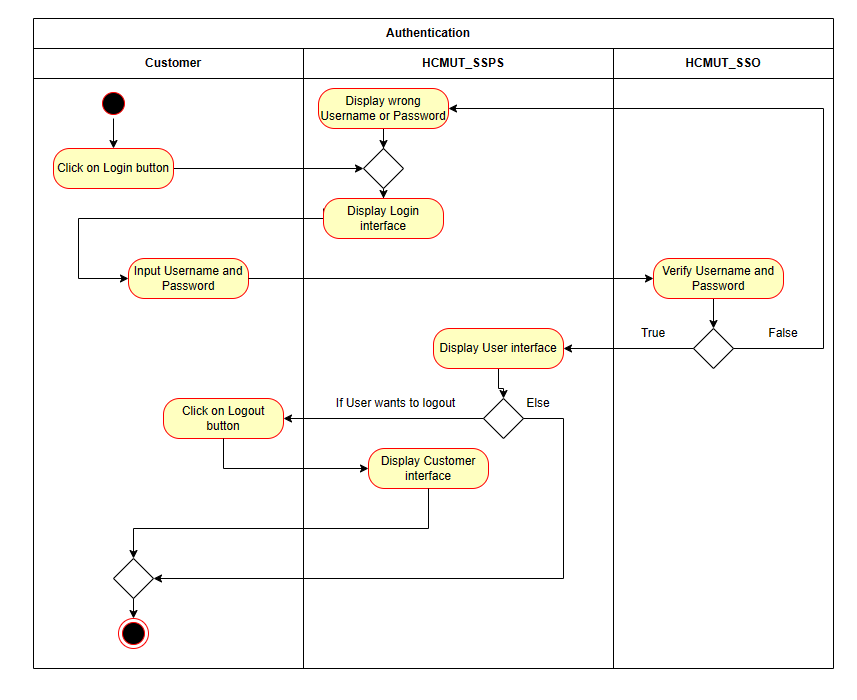
\includegraphics[width=0.9\textwidth]{Images/System Modelling/Authen_Activity.png}
        \caption{Activity diagram cho module xác thực tài khoản}
        \label{fig:arch}
    \end{center}
\end{figure}
\textbf{Mô tả:}\par
Đầu tiên, Customer chọn nút "Login", hệ thống sẽ hiển thị giao diện đăng nhập. Tại đó, Customer có thể nhập tài khoản và mật khẩu để có thể đăng nhập vào hệ thống. Sau đó hệ thống sẽ xác thực tài khoản và mật khẩu của Customer. Nếu tài khoản và mật khẩu đúng thì hệ thống sẽ hiển thị giao diện của User, nếu sai thì sẽ hiển thị tài khoản và mật khẩu sai và hiển thị lại giao diện đăng nhập. Bước tiếp theo nếu người dùng muốn đăng xuất thì chọn nút "Logout", hệ thống sẽ hiển thị giao diện của Customer.

\subsubsection{In}
\begin{figure}[H]
    \begin{center}
        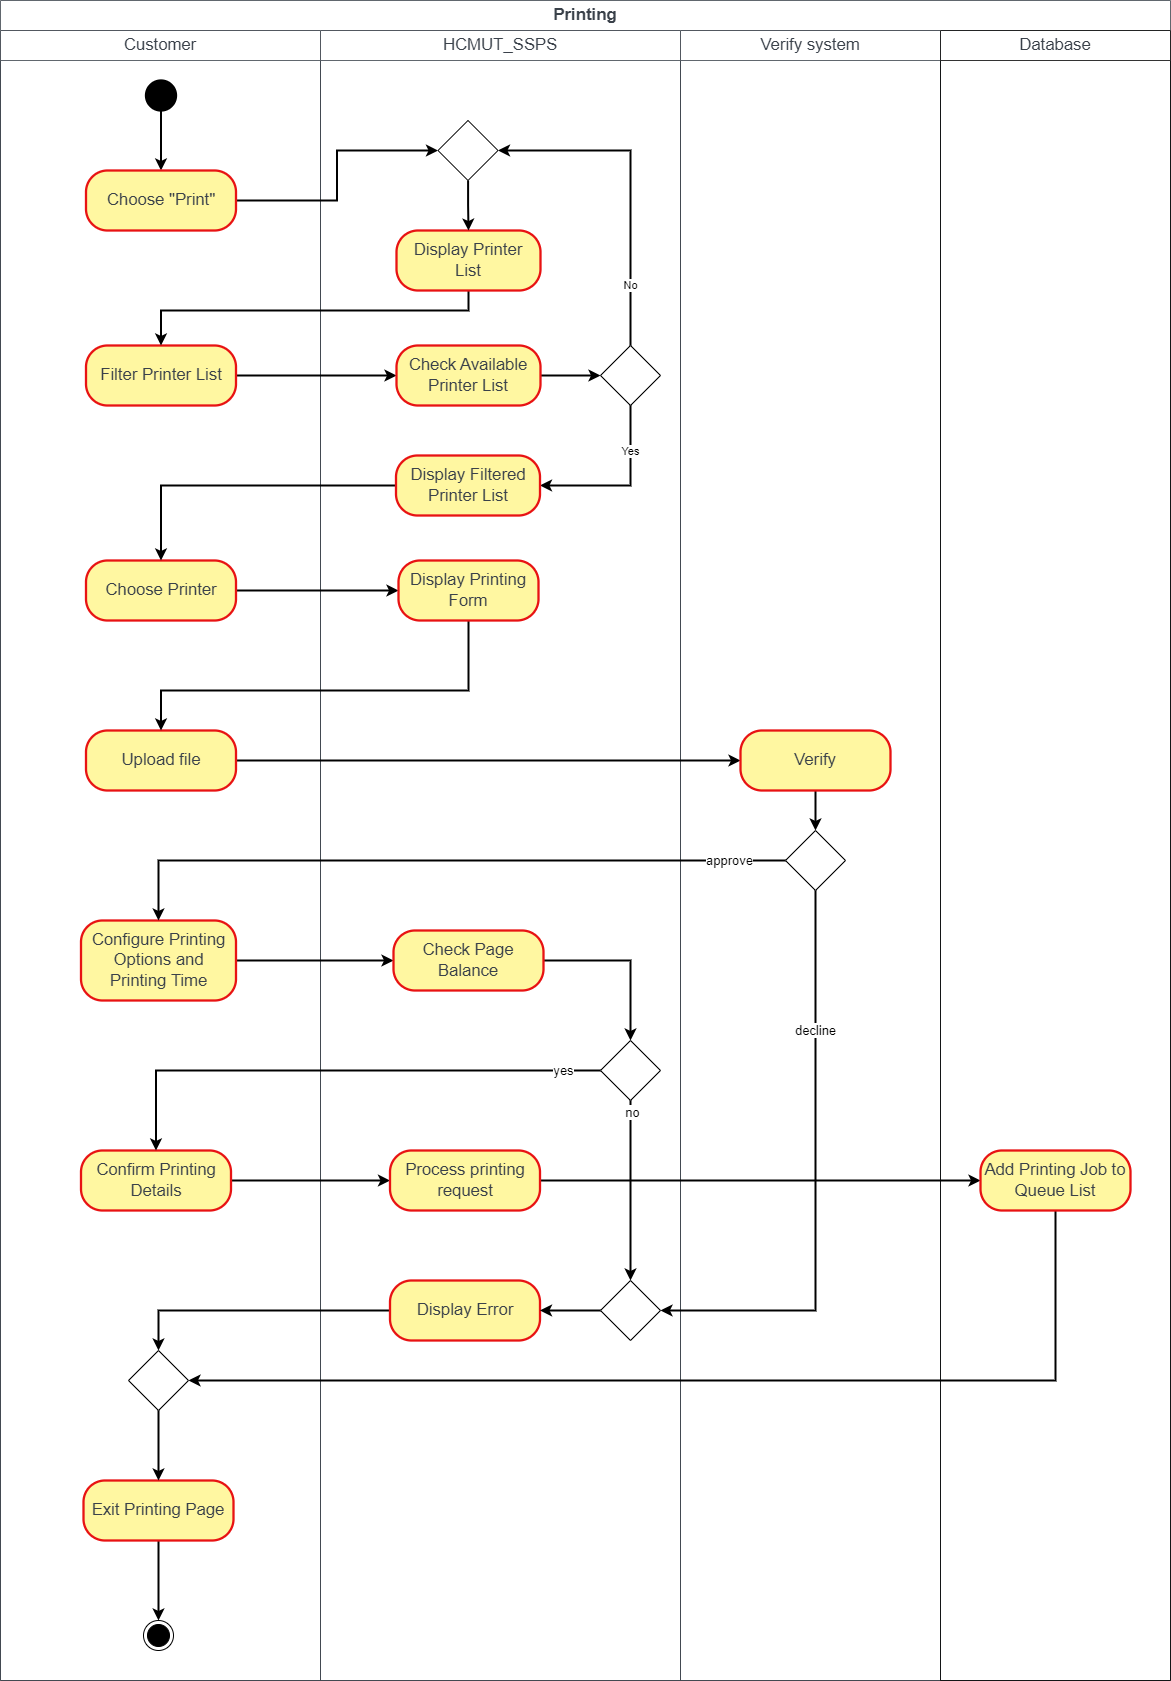
\includegraphics[width=0.8\textwidth]{Images/System Modelling/Printing_Activity.png}
        \caption{Activity diagram cho module in}
    \end{center}
\end{figure}
\textbf{Mô tả: }\par
Đầu tiên, Customer chọn nút "In ngay" trên thanh điều hướng, hệ thống sẽ hiển thị danh sách các máy in. Sau đó Customer sẽ tiến hành chọn lọc máy in bằng cách lọc cơ sở, tòa, phòng. Hệ thống sẽ kiểm tra xem những máy in thỏa mãn điều kiện lọc có đang khả thi (không bảo trì) hay không. Nếu không có máy in khả thi nào thỏa điều kiện lọc, hệ thống sẽ quay về hiển thị danh sách máy in, ngược lại hệ thống sẽ hiển thị danh sách máy in thỏa điều kiện lọc. Tại đây Customer sẽ tiến hành chọn máy in, sau đó hệ thống sẽ hiển thị form và Customer sẽ tiến hành upload file cần in lên hệ thống. Hệ thống xác thực nội dung sẽ kiểm tra file có hợp lệ hay không. Nếu file không hợp lệ, hệ thống sẽ báo lỗi về màn hình. Ngược lại, hệ thống xác thực nội dung thành công, Customer sẽ điền thông tin về số trang cần in, thời gian in, định dạng cách in. Và hệ thống sẽ kiểm tra xem số giấy Customer cần in có đủ hay không. Nếu không thì sẽ báo lỗi về Customer, và Customer cần phải giảm số trang giấy cần in hoặc mua thêm giấy. Ngược lại, Customer sẽ xác nhận thao tác in của mình và hệ thống sẽ xử lý, sau đó thêm thông tin in của Customer vào hàng chờ để xử lý.

\subsubsection{Mua giấy}
\begin{figure}[H]
    \begin{center}
        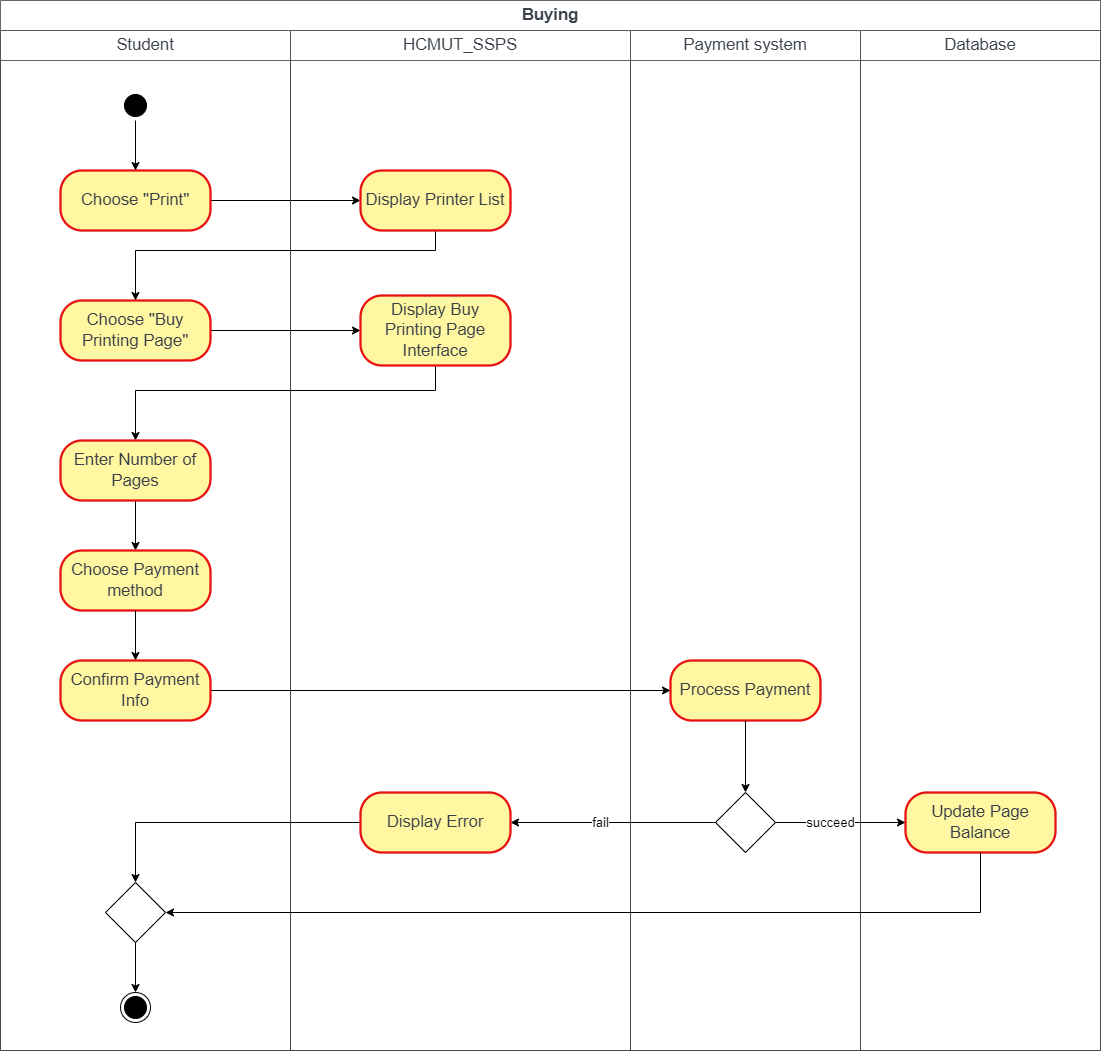
\includegraphics[width=0.7\textwidth]{Images/System Modelling/Buying_Activity.png}
        \caption{Activity diagram cho use-case mua giấy}
    \end{center}
\end{figure}
\textbf{Mô tả: }\par
Tại giao diện "In ngay", sinh viên chọn vào "Mua giấy", hệ thống sẽ hiển thị giao diện mua giấy. Tiếp theo, sinh viên sẽ nhập số lượng giấy cần mua và chọn phương thức thanh toán. Sau đó hệ thống thanh toán sẽ xử lý giao dịch, nếu thất bại thì hệ thống sẽ báo lỗi về màn hình, ngược lại dữ liệu về lượng giấy của sinh viên sẽ được cập nhật.

\subsubsection{Quản lý máy in}
\begin{figure}[H]
    \begin{center}
        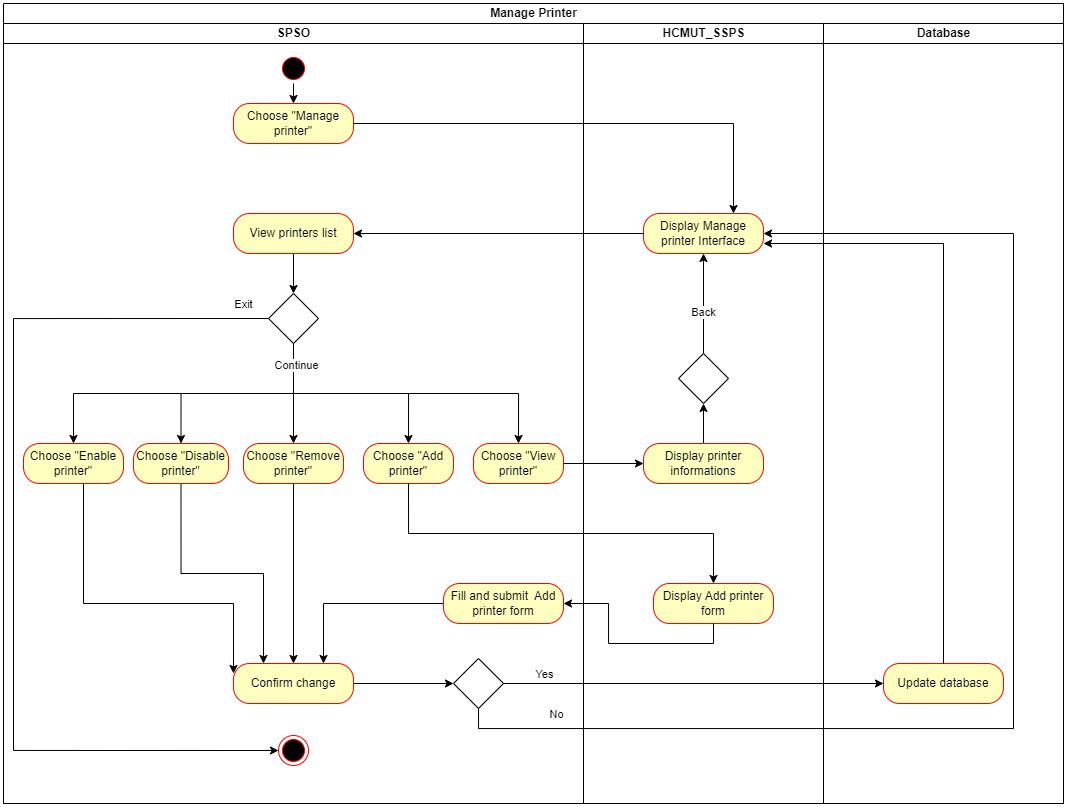
\includegraphics[width=0.9\textwidth]{Images/System Modelling/PM_Activity.png}
        \caption{Activity diagram cho module quản lý máy in}
        \label{fig:arch}
    \end{center}
\end{figure}
\textbf{Mô tả:}\par
Đầu tiên, SPSO chọn "Quản lý máy in", hệ thống sẽ hiển thị giao diện quản lý máy in và SPSO sẽ được xem danh sách các máy in. Tại đó, SPSO có thể chọn "Enable printer" để cấp phép máy in, chọn "Disable printer" để vô hiệu hóa máy in, chọn "Remmove printer" để xóa máy in hoặc có thể thêm máy in bằng cách chọn "Add printer" rồi hệ thống sẽ hiển thị form thông tin của máy in mới và SPSO phải điền và nhấn lưu. Sau các thao tác trên, SPSO phải thực hiện xác nhận thay đổi, nếu đồng ý thì dữ liệu sẽ được cập nhật và hiển thị lại danh sách máy in hoặc không thì sẽ bỏ qua và hiển thị lại danh sách máy in. Ngoài ra, khi xem danh sách máy in, SPSO còn có thể ấn nút "View printer" để xem thông tin của một máy in. Khi đó, hệ thống sẽ hiển thị các thông tin của máy in đó, nếu SPSO nhất "BacK" thì sẽ quay lại giao diện hiển thị danh sách các máy in. Tất cả các tùy chọn đều trả lại giao diện hiển thị danh sách các máy in và người dùng có thể xem. Nếu muốn tiếp tục thực hiện các tùy chọn đó thì cứ tiếp tục, còn không sẽ kết thúc hoạt động. 


\subsubsection{Sửa danh mục định dạng tệp cho phép in}
\begin{figure}[H]
    \begin{center}
        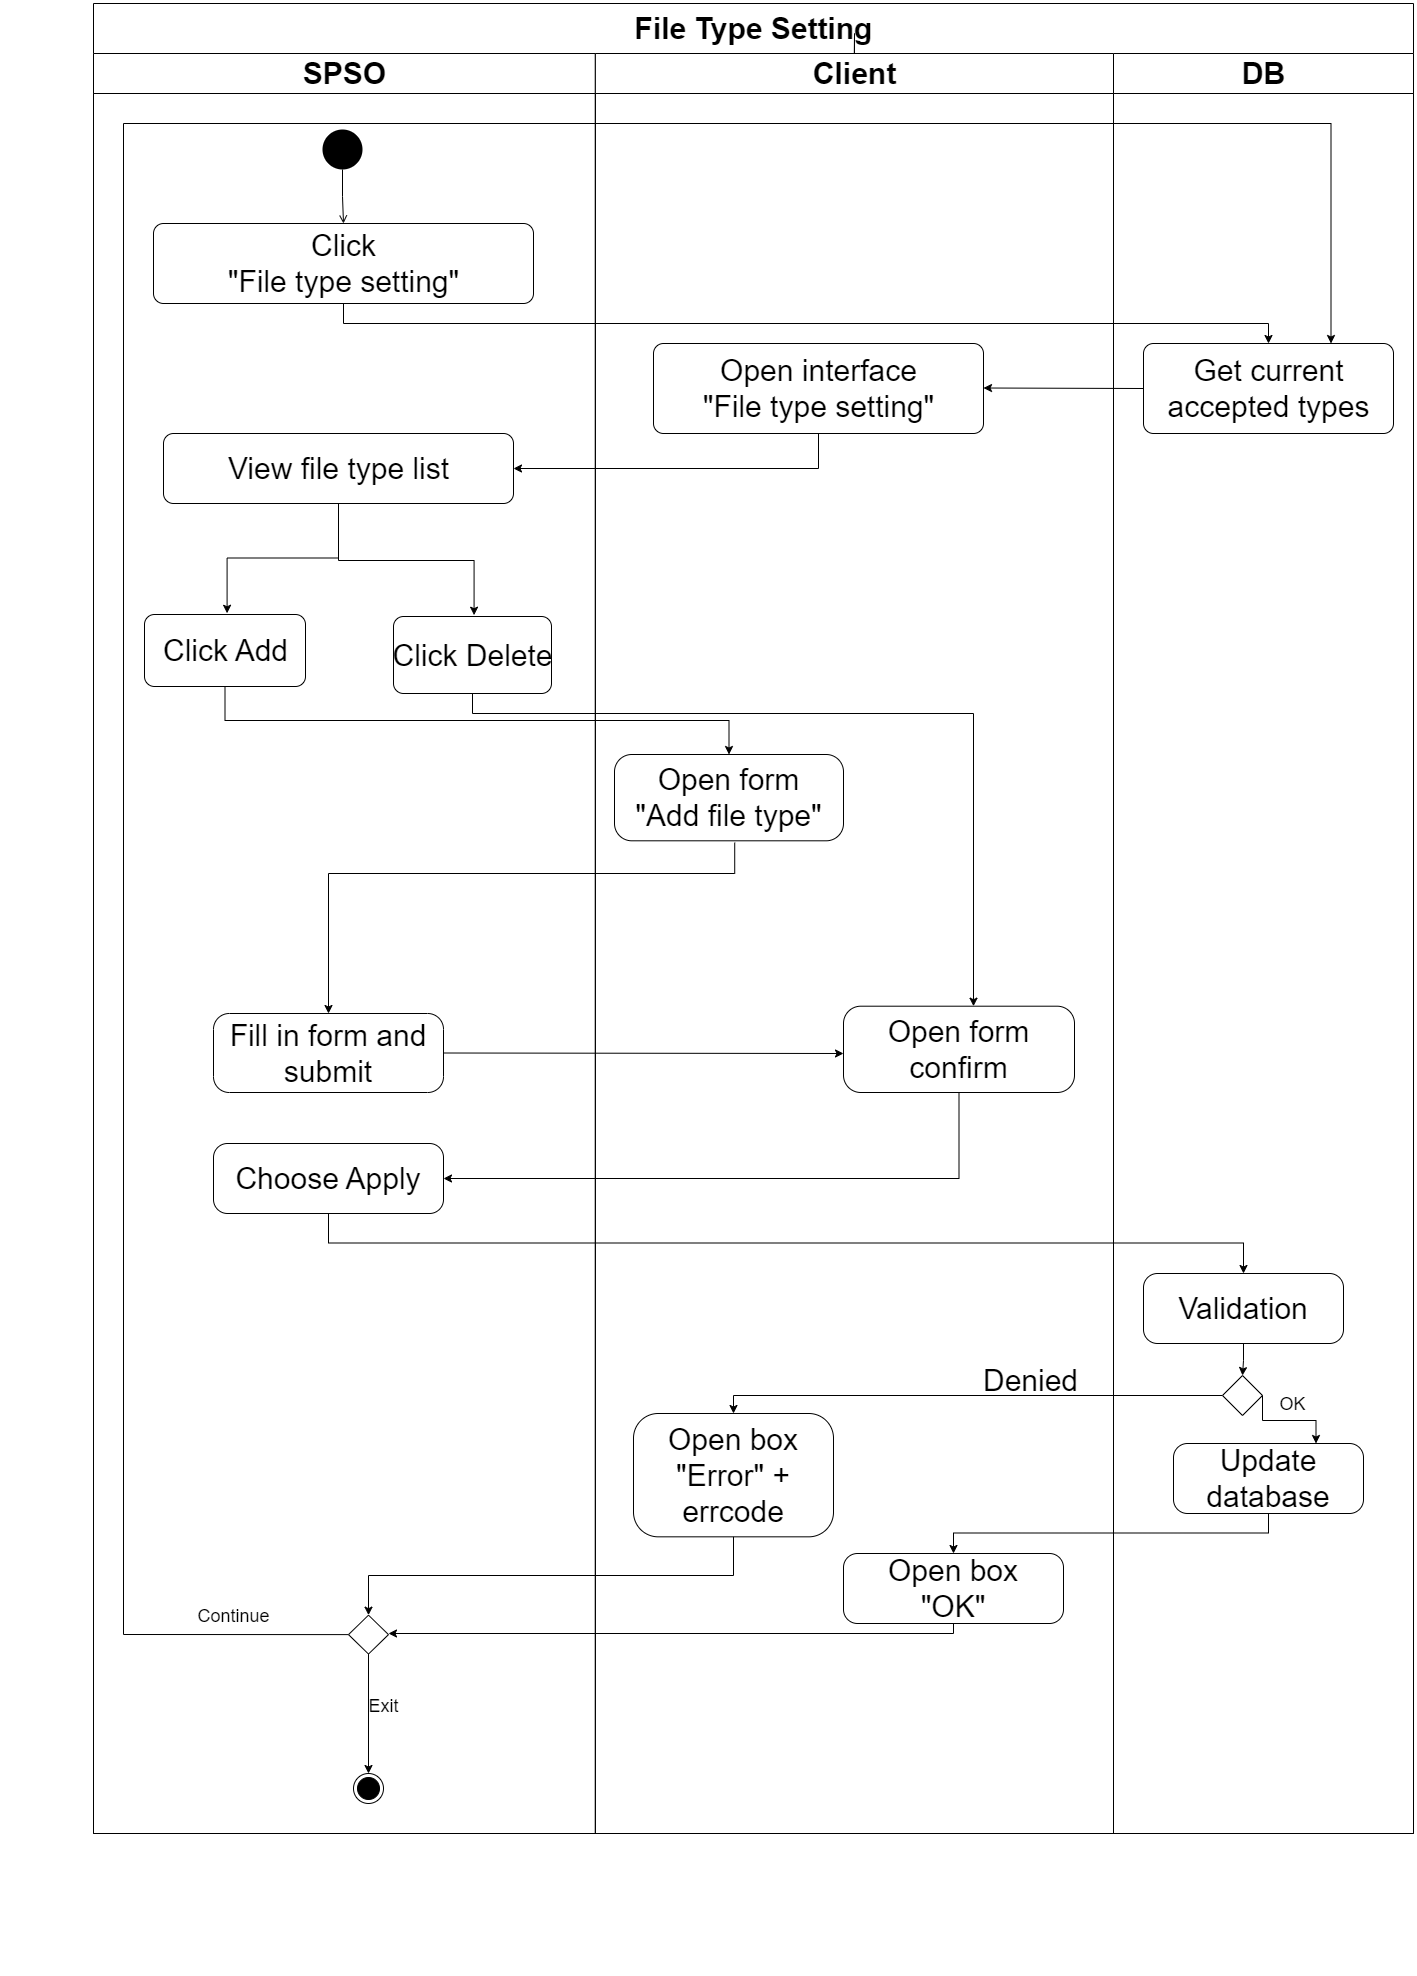
\includegraphics[width=0.7\textwidth]{Images/System Modelling/FileTypeSetting_Activity.png}
        \caption{Activity diagram cho module Sửa định dạng tệp cho phép in}
        \label{fig:arch}
    \end{center}
\end{figure}

\textbf{Mô tả:}\par
Bắt đầu, SPSO chọn "File type setting", sau đó cơ sở dữ liệu thực hiện tải những kiểu tệp được cho phép in hiện tại, và hiển thị chúng đồng thời với cửa sổ "File type setting" thông qua client. \par
Tiếp theo, SPSO xem danh sách kiểu tệp được in và quyết định thao tác chọn "Add" hoặc "Delete". Nếu chọn "Add", cửa sổ "Add file type" được hiển thị, người dùng tiếp tục nhập kiểu tệp muốn thay đổi và nhấn "Apply". Còn nếu chọn "Delete" thì chỉ cần nhấn "Apply".\par
Nếu cơ sở dữ liệu kiểm tra thay đổi hợp lệ thì cập nhật dữ liệu, sau đó client sẽ hiển thị "Ok". Nếu không hợp lệ thì không cập nhật và client báo lỗi.\par
Để kết thúc, người dùng thao tác chọn "Exit" hoặc có thể tiếp tục ở giao diện chỉnh sửa loại tệp cho phép in.

\subsubsection{Quản lý tặng giấy miễn phí}
\begin{figure}[H]
    \begin{center}
        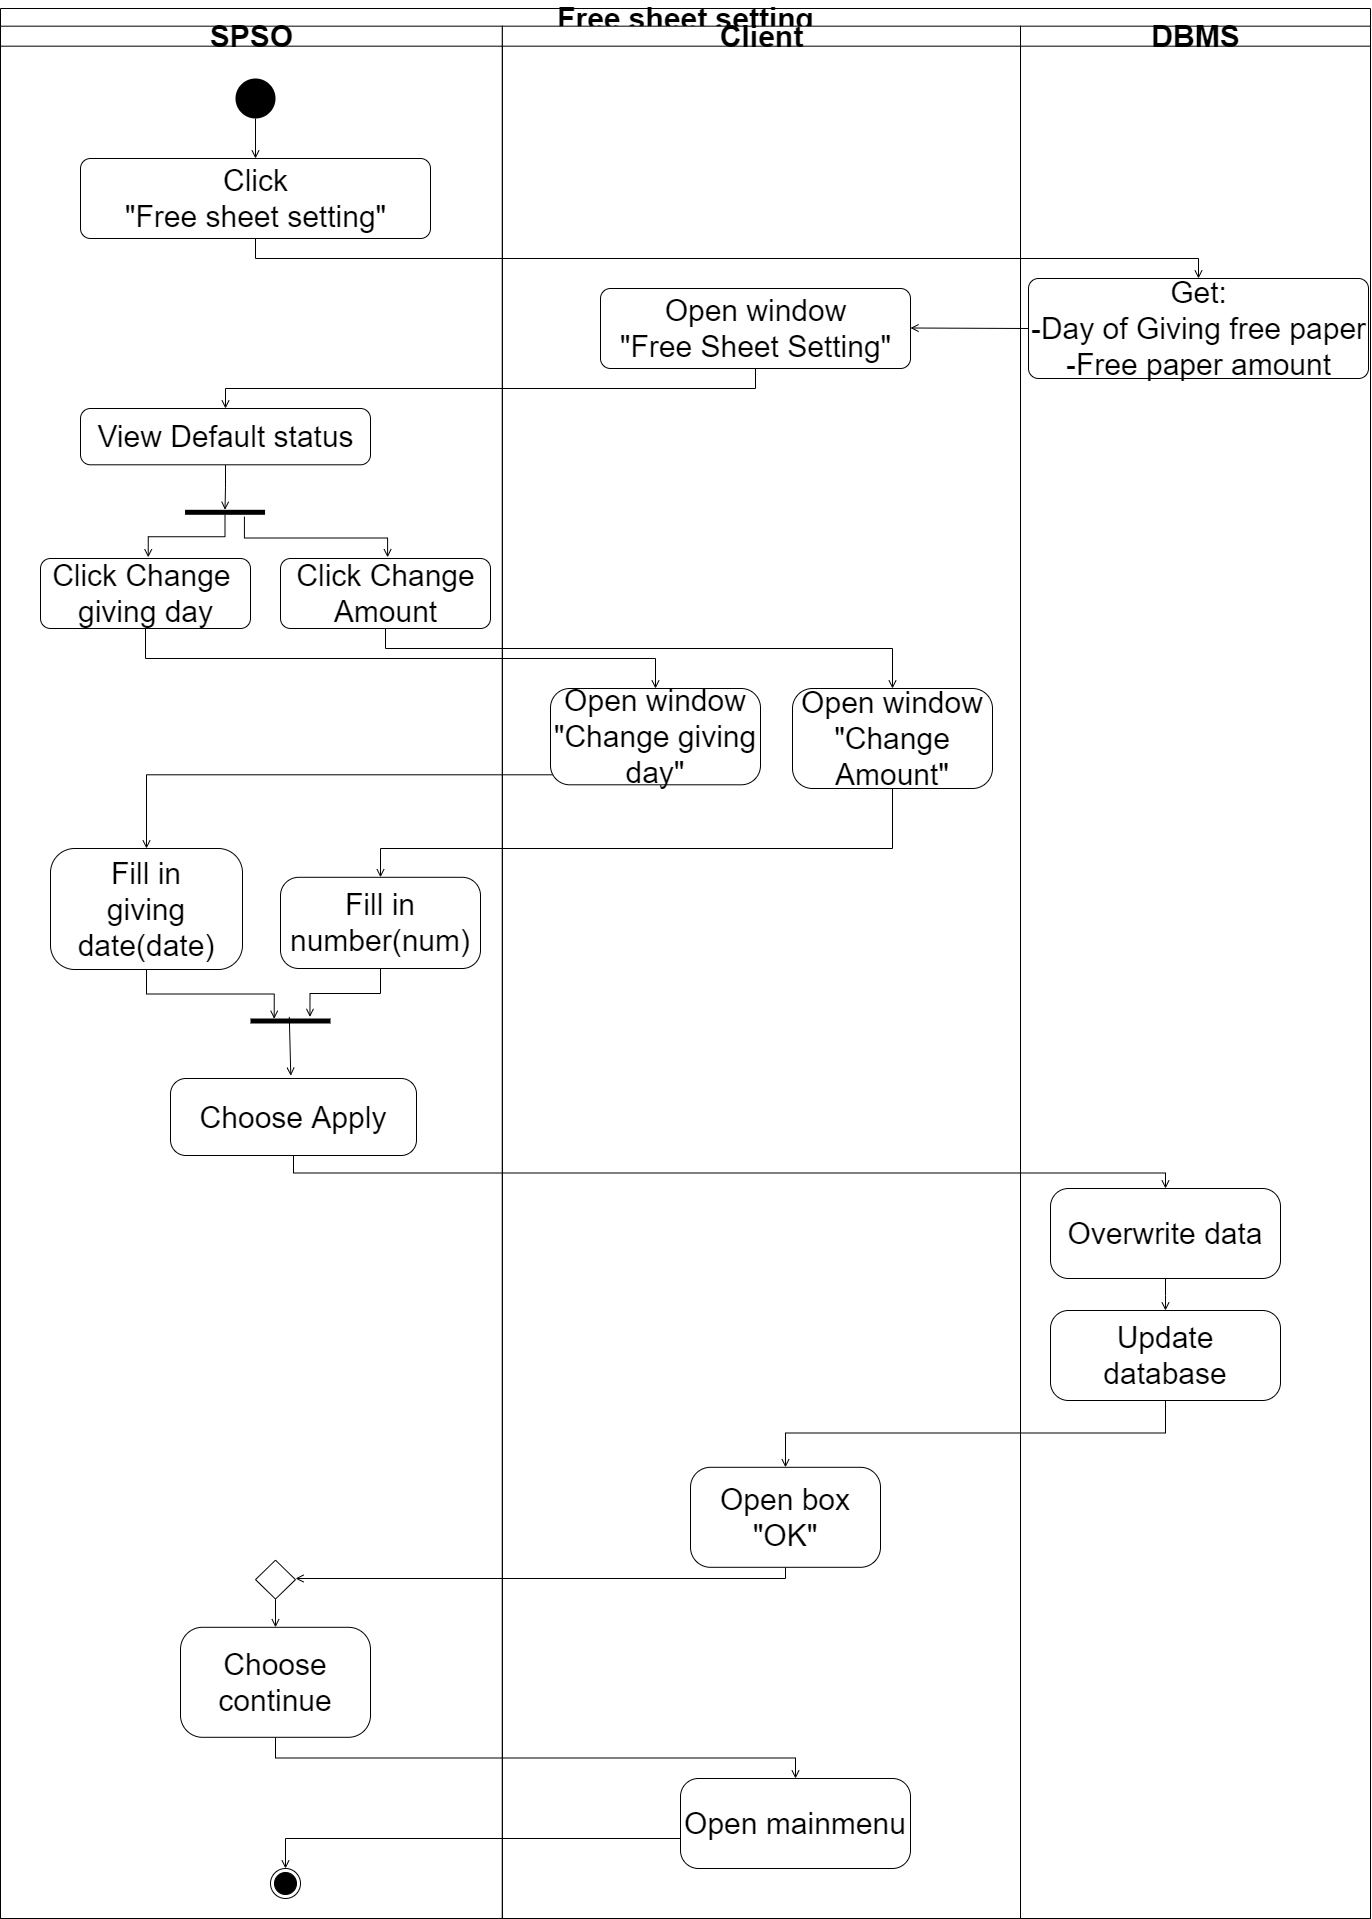
\includegraphics[width=0.7\textwidth]{Images/System Modelling/FreeSheetSetting_Activity.png}
        \caption{Activity diagram cho module Quản lý tặng giấy miễn phí}
        \label{fig:arch}
    \end{center}
\end{figure}

\textbf{Mô tả:}\par
Bắt đầu, SPSO chọn "Free sheet setting", sau đó cơ sở dữ liệu thực hiện tải trạng thái ngày phát giấy miễn phí, số lượng của giấy miễn phí hiện tại, và hiển thị chúng đồng thời với cửa sổ "Free sheet setting" thông qua client. \par
Tiếp theo, SPSO xem và chọn "Edit". Khi đó cửa sổ "Edit" được hiển thị, người dùng thực hiện thay đổi (Ngày hoặc số tờ giấy) và nhấn "Apply".\par
Nếu cơ sở dữ liệu kiểm tra thay đổi hợp lệ thì cập nhật dữ liệu, sau đó client sẽ hiển thị "Ok". Nếu không hợp lệ thì không cập nhật và client báo lỗi.\par
Để kết thúc, người dùng thao tác chọn "Exit" hoặc có thể tiếp tục ở giao diện cài đặt tặng giấy.

\subsubsection{Lịch sử in}
\begin{figure}[H]
    \begin{center}
        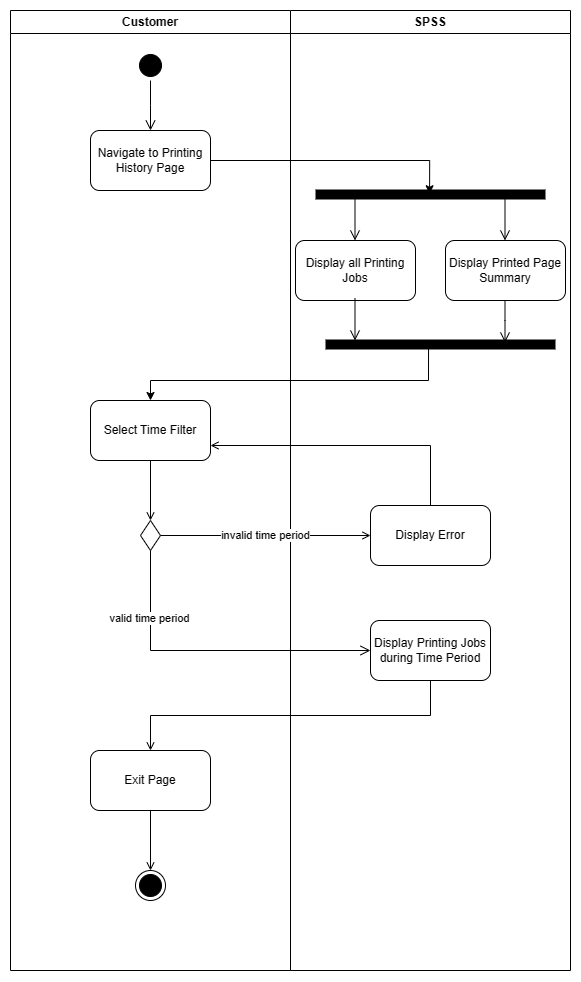
\includegraphics[width=1\textwidth]{Images/System Modelling/Logging(customer)_Activity.png}
        \caption{Activity diagram cho use case truy cập lịch sử in của Khách hàng}
        \label{fig:arch}
    \end{center}
\end{figure}
\textbf{Mô tả:}\par
Đầu tiên, khách hàng điều hướng đến trang Lịch sử in. Hệ thống sẽ hiển thị tất cả lịch sử in ấn của khách hàng đó. Khách hàng có thể chọn bộ lọc để lọc bớt dữ liệu. Cuối cùng, người dùng xem các thông tin cần thiết và thoát trang Lịch sử in.

\begin{figure}[H]
    \begin{center}
        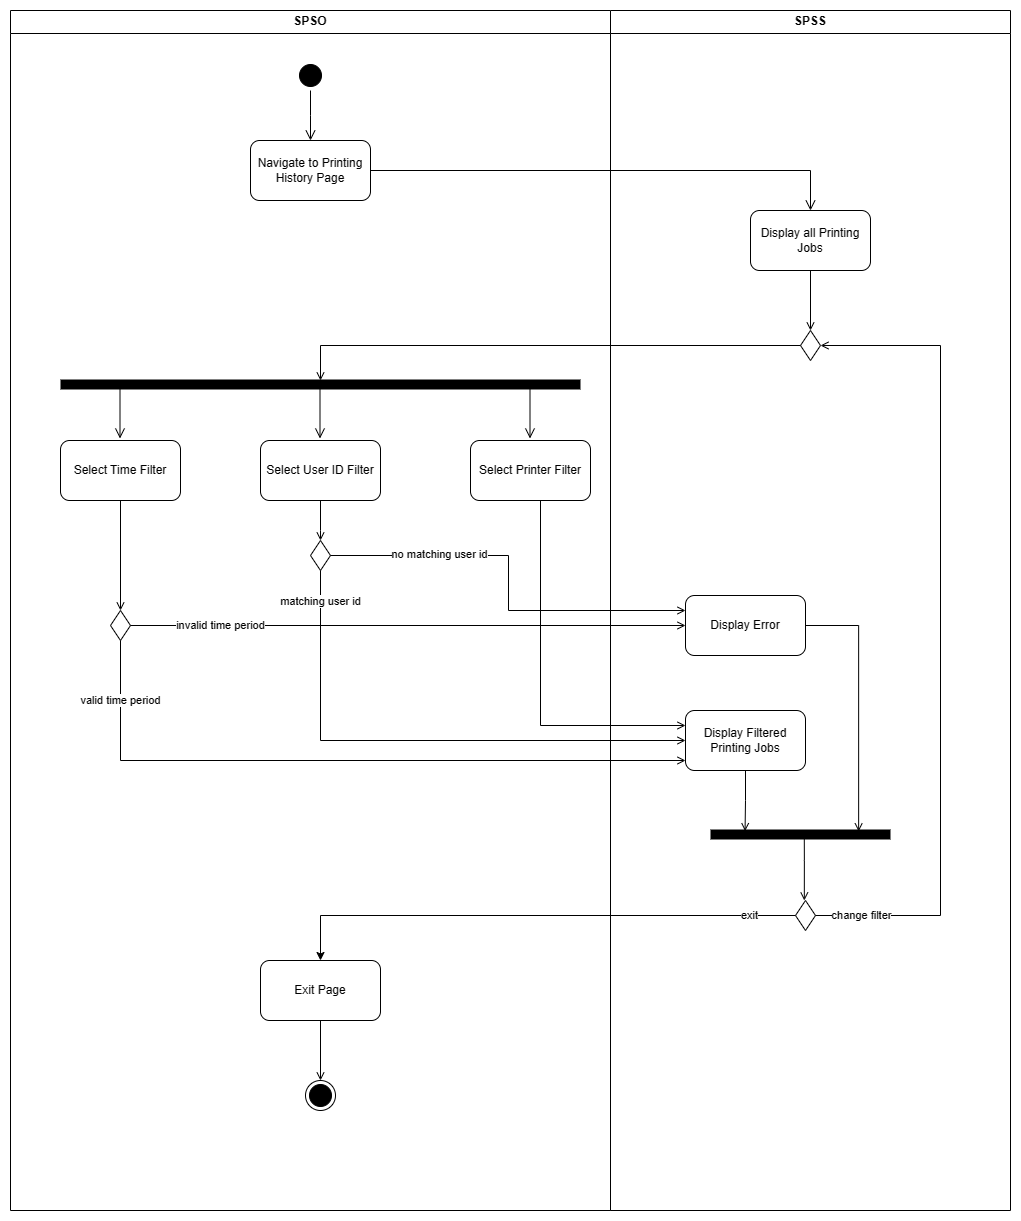
\includegraphics[width=1\textwidth]{Images/System Modelling/Logging(SPSO)_Activity.png}
        \caption{Activity diagram cho use case truy cập lịch sử in của SPSO}
        \label{fig:arch}
    \end{center}
\end{figure}

\textbf{Mô tả:}\par
Đầu tiên, SPSO điều hướng đến trang Lịch sử in. Hệ thống sẽ hiển thị tất cả lịch sử in ấn của tất cả khách hàng. Khách hàng có thể chọn bộ lọc để lọc bớt dữ liệu. Cuối cùng, SPSO xem các thông tin cần thiết và thoát trang Lịch sử in.
